\documentclass[12pt,a4paper]{article}
\title{ \line(1,0){250}
\\\sc\Large Honors Mathematics
\\\normalsize\sc(VV285)
\\UM-SJTU Joint Institute
\\\line(1,0){250}}
\usepackage{color}
\usepackage{graphicx}
\usepackage{amsmath}
\usepackage{amssymb}
\usepackage{indentfirst}
\usepackage{geometry}
\usepackage{caption}
\usepackage{float}
\usepackage{enumerate}
\usepackage{listings}
\usepackage{textcomp}
\setcounter{page}{1}
\pagenumbering{arabic}
\begin{document}
 \maketitle
 \thispagestyle{empty}

 \begin{center}
~\\
~\\
~\\ 
 \LARGE\sc
 Term Project\\
 ~\\
  \LARGE Option 1: A Perfect Pendulum\\
~\\
 ~\\
 ~\\
 ~\\

\rm \Large 
Group:19\\
~\\
\large
Ding Shuangrui \qquad 517370910194\\
Liu Zhiyuan  \qquad \quad \ 517370910240 \\
Wu Qirui \qquad  \qquad \ \  517021910681\\
Sun Yan  \qquad \qquad \quad 517370910147 \\
Sun Yi  \qquad \qquad \quad \; 517021910187 \\
\end{center} 
\newpage
~\\
\Large \textbf{ABSTRACT}\\
\normalsize
~\\
\qquad This project mainly deals with the famous mathematical tautochrone problem (also called the isochrone problem). We first studied properties of a mathematical pendulum by deriving the energy formula and pendulum equation. Then, we get an equation of the approximated period of a single pendulum, which depends on the initial displacement of the oscillator. The tautochrone problem is then involved, and we studied “Huygens Discovers the Isochrone” to find the solution. We studied the path, the cycloid curve and was finally able to construct a tautochronous pendulum. \\
\newpage
\tableofcontents
\newpage
\section{Introduction}
Pendulum has long been used for time-keeping and physical and engineering applications. It is well suited for the construction of clockworks because of its periodic motion and simple construction. However, problem exists since pendulums’ periods depend on the initial displacement.\\
~\\
\begin{figure}[!htbp]
    \centering
    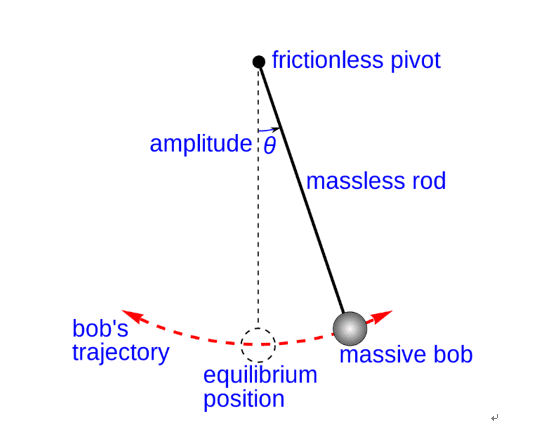
\includegraphics[scale=0.35]{intro1.png}
    \caption{A mathematical pendulum$~^{[1]}$}
    \label{1}
\end{figure}
\begin{figure}[!htbp]
    \centering
    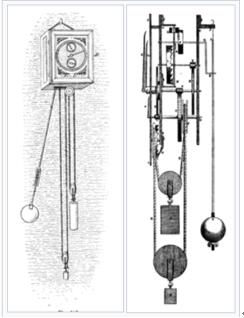
\includegraphics[scale=0.35]{intro2.jpg}
    \caption{The first pendulum clock$~^{[2]}$}
    \label{1}
\end{figure}
Hence, we did this project to solve the famous mathematical tautochrone problem (also called the isochrone problem).\\
~\\
To find the solution, we learned “Huygens Discovers the Isochrone”. The objectives of this project are listed as follows:
\begin{itemize}  
\item Learn the properties of a mathematical pendulum, i.e., derive the energy formula and pendulum equation.
\item Find the approximate period of a mathematical pendulum, which depends on the initial position of the particle.
\item Study the path of a tautochrone.
\item Find parametric equations of the cycloid curve of the tautochrone.
\item Find a way to construct a tautochronous pendulum.
\end{itemize} 
\begin{figure}[!htbp]
    \centering
    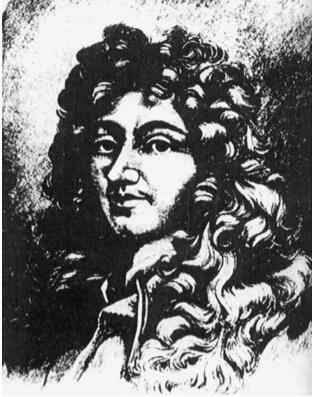
\includegraphics[scale=0.35]{intro3.jpg}
    \caption{Huygens}
    \label{1}
\end{figure}
\begin{figure}[!htbp]
    \centering
    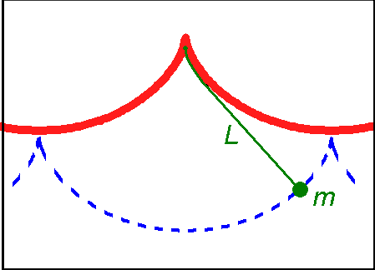
\includegraphics[scale=0.35]{intro4.png}
    \caption{Schematic of a cycloidal pendulum$~^{[3]}$}
    \label{1}
\end{figure}
In this project, mathematical knowledge we learnt in VV186 and VV285 are used, such as the Inverse Function Theorem and the elliptic integral of the first kind.\\
\section{Background}
\subsection{Mathematical Pendulum}
Mathetical pendulums are widely used in clockworks. The detailed definition will be given in the Solution section.\\
~\\
The energy of a mathematical pendulum can be expressed in the following equation:
$$E(\theta,\dot{\theta})=\frac{1}{2}ml^2 \dot{\theta}^2+ mgl(1-cos \theta)$$
where $\theta$ is the angular displacement and $\dot{\theta} $ is its time-derivative.\\
~\\
For a single period,
$$T=4\sqrt{\frac{l}{g}} \int_{0}^{\frac{\pi}{2}}\frac{d\phi}{\sqrt{1-sin^2(\theta_0/2)sin^2\phi}}$$
where $\theta_0$ is the initial amplitude.\\
~\\
We can find the approximate value by the following equation:
$$T \approx 2\pi \\sqrt{frac{l}{g}}(1+\frac{\theta_0^2}{16})\approx 2\pi \sqrt{\frac{l}{g}}$$
the right part only applies when $\theta_0 \leqslant 10^o$.\\
\subsection{The Tautochrone Problem}
The tautochrone problem was solved by Christiaan Huygens in 1659. He proved in 1673 that the curve was a cycloid.\\
~\\
A tautochrone curve is such a curve that the time taken by an object sliding without friction in uniform gravity to its lowest point is independent of its starting point. The time is equal to π times the square root of the radius over the acceleration of gravity. It can be expressed in the following equation:
$$T=\pi \sqrt{\frac{r}{g}}$$
Further details of the tautochrone problem will be explored in the Solution section.\\
\section{Analysis and Calculation}
\subsection{Mathematical Pendulum and Physical Pendulum}
\subsubsection{The definition of a Mathematical Pendulum} 
A mathematical pendulum is a particle connected by a rigid, weightless rod (or a thread) to a base by means of a pin joint that can oscillate and rotate in a plane $^{[6]}$. The rod is also assumed to be non-elastic and the air viscosity on the mass is negligible $^{[7]}$. A mathematical pendulum is often called a simple pendulum. \\
~\\
\subsubsection{The definition of a Physical Pendulum} 
For any rigid body which is pivoted so that it can oscillate freely, it is a physical pendulum $~^{[7]}$. Physical pendulum undergoes fixed axis rotation about a fixed point $~^{[8]}$ and it is often called a compound pendulum.\\
~\\
\subsubsection{The features of a Physical Pendulum $^{[8]}$} 
In this part, we will give a brief introduction about the features of the physical pendulum and compare it with a mathematical pendulum.\\
~\\
\begin{figure}[H]
\centering
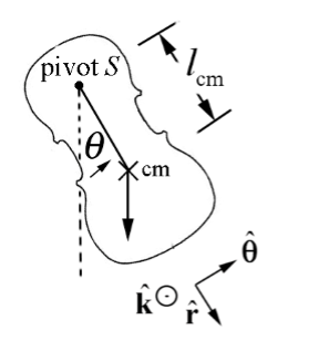
\includegraphics{1-1.png}
\caption{Physics Pendulum}
\end{figure} 
The rotation equation for a physical pendulum is:

$$I_s\frac{d^2\theta}{dt^2}+mgl_{cm}(sin\theta(t))=0$$
Here $l_{cm}$ denotes the distance from the center of mass to the pivot point S and $I_s$ is the moment of inertial about the pivot point S.\\
~\\
The period of a physical pendulum is :
$$T\approx 2\pi\sqrt{\frac{I_s}{mgl_{cm}}}$$
\subsubsection{Difference between Mathematical Pendulum and Physical Pendulum}
We use a table to show the difference between mathematical pendulum and physical pendulum:
\begin{table}[h!]
\centering
\begin{tabular}{|c|c|c|}
\hline
~&Mathematical Pendulum&Physical Pendulum\\
\hline
Rotation equation&$ml^2\frac{d^2\theta}{dt^2} $+mglsin($\theta(t)$)=0&$I_s\frac{d^2\theta}{dt^2} $+$mgl_{cm}$sin($\theta(t)$)=0\\
\hline
Period&T $\approx 2\pi \sqrt{\frac{l}{g}}$&T $\approx 2\pi \sqrt{\frac{l_{cm}}{g}+\frac{I_{cm}}{mgl_{cm}}}$\\
\hline
Object&Particle&Rigid Body\\
\hline
Radius of gyration&Constant&Not constant\\
\hline
\end{tabular}
\end{table}
\subsubsection{Further Exploration$^{[8]}$}
If we use the parallel axis theorem in the period equation for a physical pendulum and replace $I_s$ in it, then we will get:
$$I_s=ml_{cm}^2+I_{cm}$$
$$T \approx 2\pi \sqrt{\frac{l_{cm}}{g}+\frac{I_{cm}}{mgl_{cm}}}$$
Here $I_{cm}$ is the moment of inertial about the center of mass.\\
~\\
If the object is small enough and satisfies $I_{cm} \ll$ $ml_{cm}^2$, then the equation for the period can be rewritten as:
$$T \approx 2\pi \sqrt{\frac{l_{cm}}{g}}$$
which reduces to the equation for a mathematical pendulum.\\
~\\
This gives us some hints that a physical pendulum is just an extension of a mathematical pendulum.\\
\subsection{Energy of a Mathematical Pendulum}
\begin{figure}[H]
\centering
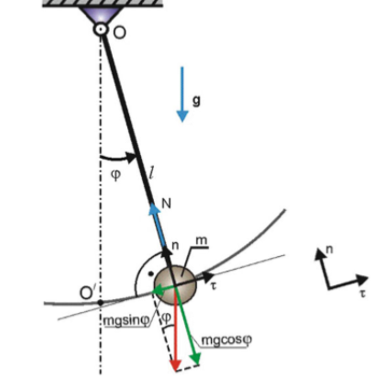
\includegraphics{1-2.png}
\caption{Mathematical Pendulum}
\end{figure} 
We choose the place where the tension in the rod is equal to the weight of the particle as the equilibrium position and denote this place with O. The length of the rod is l. The particle is with mass m. $\theta$ denotes the angle the pendulum forms with respect to the vertical direction. In our discussion, we choose the equilibrium position as the position which has zero potential energy.\\
~\\
The total energy of a particle is given by:
$$E_{total}=K+U$$
While K is the kinetic energy and U is the potential energy. K can be expressed as:
$$K=\frac{1}{2}mv^2$$
Here v is the linear velocity and because we have a rotation motion here, thus we have:
$$v=\omega l=\frac{d\theta}{dt}*l=\dot{\theta}l$$
Here $\dot{\theta}$ is a time-derivative function of $\theta$.\\
Hence the kinetic energy can be expressed as:
$$K=\frac{1}{2}m \dot{\theta}^2l^2$$
The change in the height is given by:
$$h=l-lcos\theta$$
so that the potential energy is:
$$U=mgl(1-cos \theta)$$
Hence, the total energy of the particle depends on the $\theta$ and  $\dot{\theta}$ so we can write the energy of a mathematical pendulum in the form:
$$E(\theta,\dot{\theta})=\frac{1}{2}m\dot{\theta}^2l^2+mgl(1-cos\theta)$$
Since there are only gravitational force and tension in the rod in this system. The tension in the rod doesn’t do any work and the gravitational force is a conservative force, so the total mechanical energy of the mathematical pendulum is conservative and is a constant, so we can simply differentiate the above equation with respect to t and get:\\
$$\frac{dE(\theta,\dot{\theta})}{dt}=\frac{1}{2}m(2\dot{\theta}\ddot{\theta}l^2+mglsin\theta\dot{\theta}=0)$$
Divide m , the square of l and $\dot(\theta)$ in both sides, and since $\theta$ also depends on t, we get:
\begin{equation}
\ddot{\theta}+\frac{g}{l}sin(\theta(t))=0
\end{equation}
\subsection{Period of a Pendulum}
According to the $pendulum$ $equation$
$$\frac{d^2\theta(t)}{dt^2}+\frac{g}{l}sin(\theta(t))=0$$
What's more,
$$\frac{d}{dt}(\frac{d\theta}{dt})=\frac{d\dot \theta}{dt}=\frac{d\dot \theta}{d\theta}\frac{d\theta}{dt}=\frac{1}{2}\frac{d(\dot {\theta^2)}}{d\theta}$$
We can get:
$$\frac{1}{2}\frac{d(\dot \theta)^2}{d\theta}=-\frac{g}{l}sin(\theta(t))$$
Separate the variable $d(\dot \theta)^2$ and $d\theta$, and integrate on both sides.
$$\int_0^{\dot \theta^2} d(\dot{ \theta^2})=\int_{\theta_0}^\theta-\frac{2g}{l}sin(\theta)d\theta$$
$$\dot \theta^2=\frac{2g}{l}(cos(\theta)-cos(\theta_0))$$
Therefore, $$|\dot \theta|=\sqrt{\frac{2g}{l}(cos(\theta)-cos(\theta_0))}$$
\begin{figure}[H]
\centering
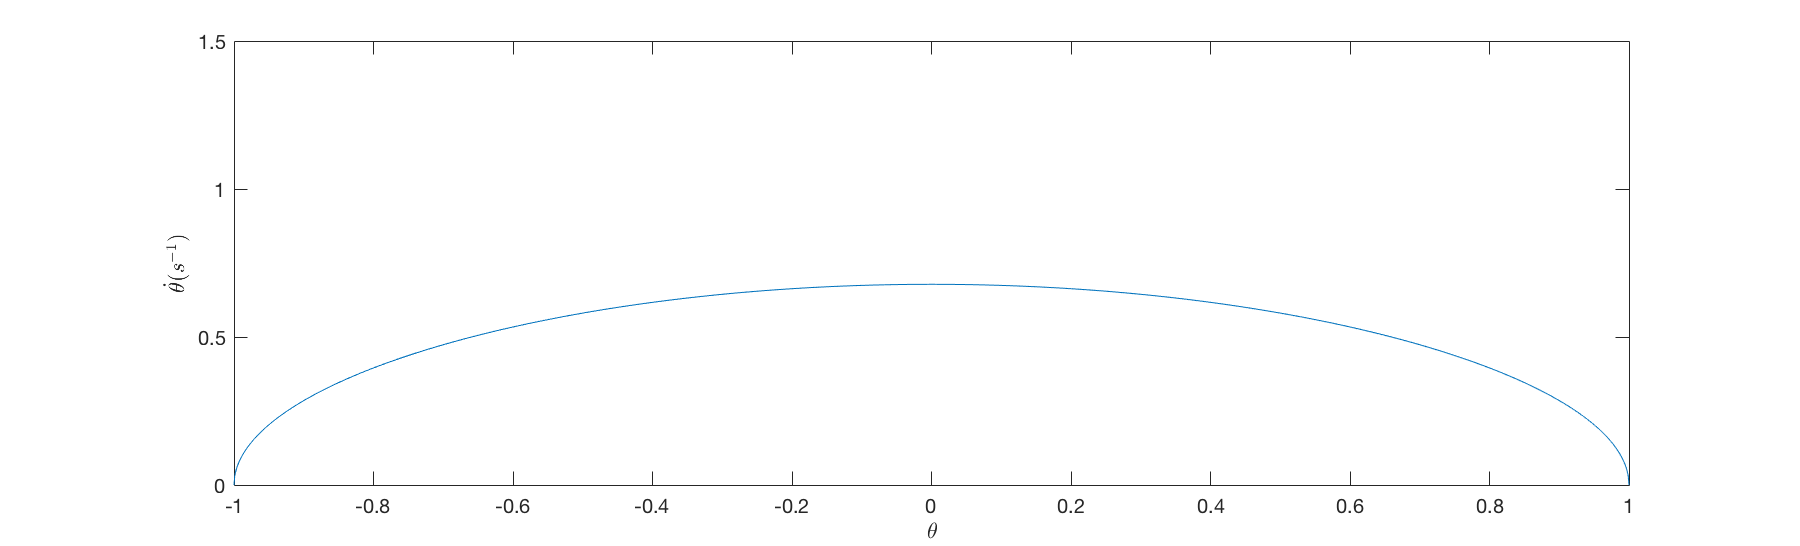
\includegraphics[width=\textwidth]{w.png}
\caption{Graph of $|\dot \theta|=\sqrt{cos(\theta)-cos(1)}$.}
\end{figure} 

As shown in the graph, since the $|\dot \theta|$ is symmetric with respect to $\theta=0$. Thus, the time cost by two sides' motion is equal, whenever it goes toward or against the middle point because the angular speed is same at every $|\theta|$.\\\\
Therefore, for a quarter of single period, the map
$$\quad t\mapsto\theta\qquad t\in[0,\frac{T}{4}]\quad \theta\in[0,\theta_0] $$ 
is bijective and hence invertible. Plus, it is also continuous and strictly decreasing.
According to the Inverse Function Theorem of Vv186,
\begin{figure}[H]
\centering
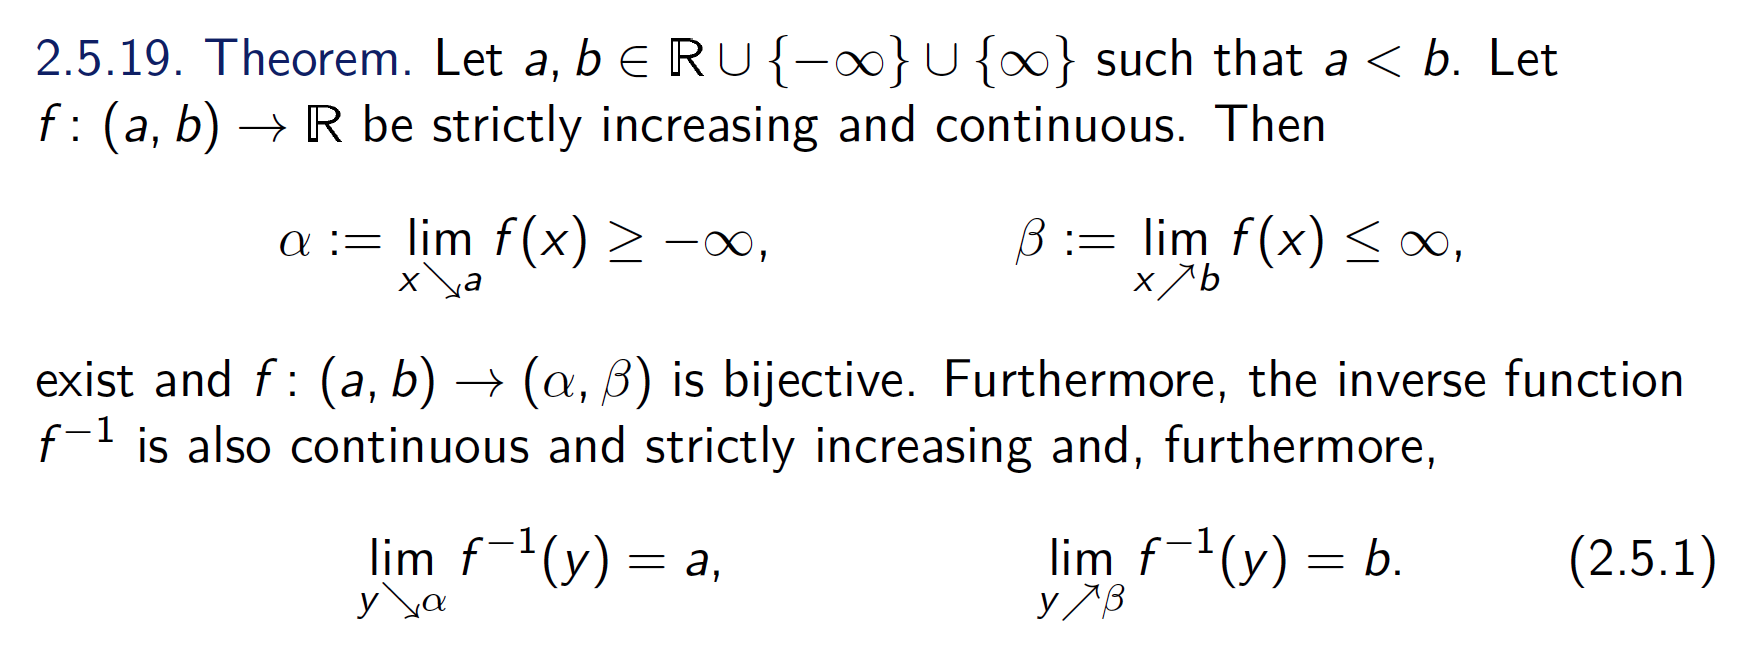
\includegraphics[width=\textwidth]{inverse.png}
\end{figure} 
We can get:
$$\quad \theta\mapsto t\qquad \theta\in[0,\theta_0]\quad t\in[0,\frac{T}{4}] $$ 
which is also continuous and strictly decreasing($\dot \theta \leq 0$).
Therefore, we can separate the variable $d\theta$ and $dt$, and integrate on both sides.
$$-\dot \theta=\sqrt{\frac{2g}{l}(cos(\theta)-cos(\theta_0))}$$
$$\int_0^{\frac{T}{4}}dt=-\int_{\theta_0}^0\frac{d \theta}{\sqrt{\frac{2g}{l}(cos(\theta)-cos(\theta_0))}}$$
$$T=4\sqrt{\frac{l}{2g}}\int_0^{\theta_0}\frac{d \theta}{\sqrt{cos(\theta)-cos(\theta_0)}}$$
Using a substitution $sin(\phi)=sin(\frac{\theta}{2})/sin(\frac{\theta_0}{2})\in[0,1]$,
$$cos(\phi)d\phi=\frac{cos(\frac{\theta}{2})}{2sin({\frac{\theta_0}{2}})}d\theta$$
Since $cos(\frac{\theta}{2})^2+sin(\frac{\theta}{2})^2=1$,
$$cos(\phi)d\phi=\frac{\sqrt{1-sin^2(\phi)sin^2(\frac{\theta_0}{2})}}{2sin({\frac{\theta_0}{2}})}d\theta$$
Substitute $\theta$ by $\phi$,
$$T=4\sqrt{\frac{l}{g}}\int_0^{\frac{\pi}{2}}\frac{d\phi}{\sqrt{1-sin^2(\phi)sin^2(\frac{\theta_0}{2})}}$$
Since it is a complete elliptic integral of the first kind, we know:
$$K(k)=\int_0^{\frac{\pi}{2}}\frac{d\phi}{\sqrt{1-k^2sin^2(\phi)}}\qquad (k=sin(\frac{\theta_0}{2}))$$
We then give the period of the pendulum in terms of the arithmetic-geometric mean,
$$K(k)=\frac{\frac{\pi}{2}}{agm(1,\sqrt{1-k^2})}$$
Therefore, we can get:
\begin{equation}
T=4\sqrt{\frac{l}{g}}\frac{\frac{\pi}{2}}{agm(1,cos(\frac{\theta_0}{2}))}
\end{equation}
where $agm(1,cos(\frac{\theta_0}{2}))$ stands for the arithmetic-geometric mean of $(1,cos(\frac{\theta_0}{2}))$.\\
Then, we can use the Taylor expansion to unfold the formula.\\
As we know, the Taylor expansion at $x_0$ is:
$$f(x)=f(x_0)+\frac{1}{1!}f^\prime(x)|_{x=x_0}(x-x_0)+\frac{1}{2!}f^{\prime \prime}(x)|_{x=x_0}(x-x_0)^2+...$$
Unfold the period's expression at $x=0$ using the Taylor expansion.
$$\frac{1}{\sqrt{1-x}}=1+\sum_{i=1}^{\infty}\frac{(2i-1)!!}{2^i}x^i=1+\frac{1}{2}x+\frac{3}{4}x^2+\frac{15}{8}x^3+....$$
Then we get:
$$T=4\sqrt{\frac{l}{g}}\int_0^{\frac{\pi}{2}}(1+\frac{1}{2}sin^2(\phi)sin^2(\frac{\theta_0}{2})+\frac{3}{4}(sin^2(\phi)sin^2(\frac{\theta_0}{2}))^2+\frac{15}{8}(sin^2(\phi)sin^2(\frac{\theta_0}{2}))^3+....)d\phi$$
$$T=4\sqrt{\frac{l}{g}}(\int_0^{\frac{\pi}{2}}d\phi+\int_0^{\frac{\pi}{2}}\frac{1}{2}sin^2(\frac{\theta_0}{2})sin^2(\phi)d\phi+\int_0^{\frac{\pi}{2}}\frac{3}{4}sin^4(\frac{\theta_0}{2})sin^4(\phi)d\phi+\int_0^{\frac{\pi}{2}}\frac{15}{8}sin^6(\frac{\theta_0}{2})sin^6(\phi)d\phi+...)$$
Since $\int_0^{\frac{\pi}{2}}sin^{2n}(\phi)d\phi=\frac{\pi}{2}\frac{(2n-1)!!}{(2n)!!}$, which can be derived by the mathematical induction, we rewrite the period equation.
$$T=4\sqrt{\frac{l}{g}}(\frac{\pi}{2}+\frac{\pi}{8}sin^2(\frac{\theta_0}{2})+\frac{9\pi}{64}sin^6(\frac{\theta_0}{2})+...)$$
$$T=2\pi\sqrt{\frac{l}{g}}(1+\frac{1}{4}sin^2(\frac{\theta_0}{2})+o(sin^2(\frac{\theta_0}{2})))\qquad as\quad sin^2(\frac{\theta_0}{2})\rightarrow 0$$
When $\theta_{0}\rightarrow 0$, $$sin(\frac{\theta_0}{2})=sin(0)+(sin(\frac{\theta_0}{2}))^\prime\frac{\theta_0}{2}|_{\frac{\theta_0}{2}=0}+o({\theta_0})=\frac{\theta_0}{2}+o({\theta_0})$$
It is not hard to get:
$$T=2\pi\sqrt{\frac{l}{g}}(1+\frac{1}{4}(\frac{\theta_0}{2})^2+o(\theta_0))\approx2\pi\sqrt{\frac{l}{g}}(1+\frac{1}{4}(\frac{\theta_0}{2})^2)$$
\begin{equation}
T\approx2\pi\sqrt{\frac{l}{g}}(1+\frac{\theta_0^2}{16})\approx2\pi\sqrt{\frac{l}{g}}
\end{equation}
\subsection{Proof of the Uniqueness of the Tautochrone}
Since we know that the unique solution of $\frac{d^2s}{dt^2}=-ks$ ($k>0$) is 
\begin{equation}
s=s_0cos(\sqrt{k}t+\phi)
\end{equation}
\begin{figure}[H]

\centering
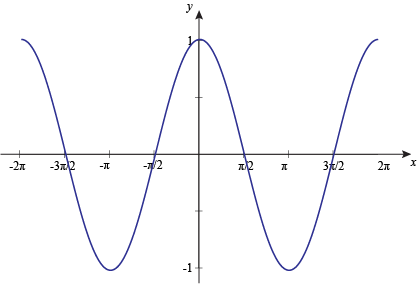
\includegraphics[width=9cm,height=5cm]{cos.png}
\caption{Cosine function when $s_{0}=1$, $k=1$ and $\phi=0$.}
\end{figure} 

The period of the motion $T=\frac{2\pi}{\sqrt{k}}$ is independent on $s_0$.
Here comes question: Is $\frac{d^2s}{dt^2}=-ks$ the only form of Tautochrone? The answer is yes.
Supposed the periodic motion can be expressed as $\frac{d^2s}{dt^2}=F(s)$.
Using some technique, we can get:
$$\frac{d}{dt}(\frac{ds}{dt})=\frac{d\dot s}{dt}=\frac{d\dot s}{ds}\frac{ds}{dt}=\frac{1}{2}\frac{d(\dot{ s^2})}{ds}=F(s)$$
Then, we separate the variable ds and $d(\dot s)^2$, and integrate on the both sides.
$$\int d(\dot {s^2})=\int 2F(s)ds$$
We define $s(0)=s_0$ and $\dot s(0)=0$, where is at the end of the path.
Then we get:
$$\int_{0}^{\dot s^2} d(\dot s^2)=\int_{s_0}^{s} 2F(s)ds$$
$$\dot s=\frac{ds}{dt}=\sqrt{\int_{s_0}^{s} 2F(s)ds}$$
In case to mistake the notation, we change slightly the equation.
$$\dot s=\frac{ds}{dt}=\sqrt{\int_{s_0}^{s} 2F(s_1)ds_1}$$
Then, we separate the variable ds and dt, and  integrate from the end to the middle point of the path.
$$\int_{s_0}^{0} \frac{ds}{\sqrt{\int_{s_0}^{s} 2F(s_1)ds_1}}=\int_0^{\frac{T}{4}} dt$$

\begin{equation}
\frac{T}{4}=\int_{s_0}^{0} \frac{ds}{\sqrt{\int_{s_0}^{s} 2F(s_1)ds_1}}
\end{equation}
Using the substitutions  $x=s_1/s_{0}$ and $y=s/s_{0}$, we insert $x,y$ into the above equation.
$$\frac{T}{4}=\int_{s_0}^{0} \frac{d(s_{0}y)}{\sqrt{\int_{s_0}^{s_{0}y} 2F(s_{0}x)d(s_{0}x)}}$$
Extract $s_{0}$ from the variable,
$$\frac{T}{4}=\int_{1}^{0} \frac{s_{0}dy}{\sqrt{s_{0}\int_{1}^{y} 2F(s_{0}x)dx}}$$
\begin{equation}
\frac{T}{4}=\int_{1}^{0} \frac{dy}{\sqrt{\int_{1}^{y} 2\frac{F(s_{0}x)}{s_0}dx}}
\end{equation}
As mentioned before, if the curve belongs to tautochrone, the period T we define is supposed to be independent on $s_0$. Looking into the equation above, we can see that only component related to $s_{0}$ is $\frac{F(s_{0}y)}{s_0}$. Thus, we can eliminate the $s_{0}$ in the equation if and only if 
$$\frac{F(s_{0}x)}{s_0}=f(x)$$
Whatever the form of f will be, there is no relation with $s_0$.
The following part is to prove the $$F(x)=-kx\quad(k>0).$$
Firstly, since the $s_{0}$ can be any value in the $R^+$, 
$$F(x)=f(x)\quad\quad when\quad s_{0}\equiv1$$
So, $F(s_{0}x) = s_{0}F(x)$.
Secondly, derivative both side with respect to x.
$$\qquad\quad\frac{dF(s_0x)}{dx}=\frac{dF(x)}{dx}$$
$$\frac{dF(s_0x)}{d(s_0x)}\frac{d(s_0x)}{dx}=s_0F^\prime(x)$$


$$\qquad\quad F^\prime(s_0x)=F^\prime(x)$$

Since the $s_{0}$ can be any value in the $R^+$, 
\begin{equation}
F^\prime(x)=const
\end{equation}
So, the form of F(x) should be proportional to x. We define:
$$F(x)=kx\quad k\in R$$\
We plug F(x) into the Eq.(6), we can get:
$$\frac{T}{4}=\int_{1}^{0} \frac{dy}{\sqrt{\int_{1}^{y^2} kd(x^2)}}$$
$$\quad=\int_{1}^{0} \frac{dy}{\sqrt{k(y^2-1)}}$$
Since $T\in R^+$ and $y=s/s_0\in [0,1]$, which means $y^2-1\leq 0$,

\begin{equation}
k<0
\end{equation}
At last, we want k to be a positive number, so we get:
$$F(x)=-kx\quad k>0$$
Therefore, the Tautochrone must be a path along which $\frac{d^2s}{dt^2}=-ks$ ($k>0$), where t is time and s is the path length.

The simple pendulum does not exactly satisfy this relation since we use some approximations to get the $\theta_0$-independent period.

\subsection{Proof of a Cycloid Curve}
The proof of a cycloid curve in this part is firstly derived from the two expressions for $\frac{d^2s}{dt^2}$. For the first part, we wish to find a path $r(t)$ such that gravity and tension in the thread combine to produce a net force whose tangential component has magnitude $kms$. Thus, according to Newton's Second Law, we can derive
$$m\frac{d^2s}{dt^2} = -kms$$
Thus, it is clear that
\begin{equation}
    \frac{d^2s}{dt^2} = -ks
\end{equation}
For the second part, we does the free body diagram for the pendulum as Figure 9, since the only force is the gravity force. The line of the bob is always vertical to the tangent line of the curve.Now we suppose the angel between the line of the bob and the vertical line is $\theta$ so we can get
\begin{figure}[!htbp]
    \centering
    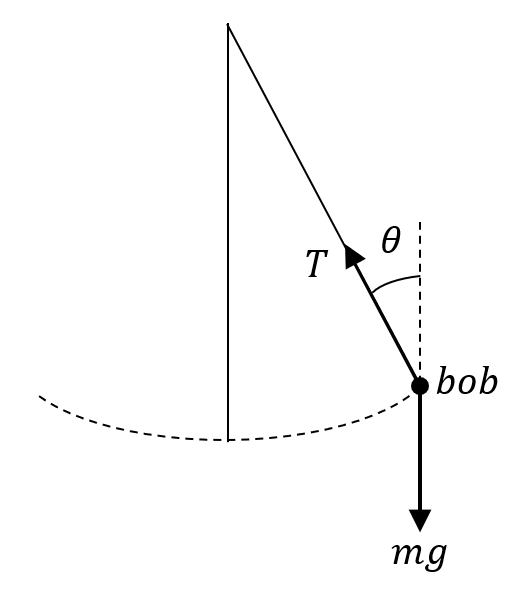
\includegraphics[scale=0.35]{1.png}
    \caption{free body diagram}
    \label{force}
\end{figure}
$$m\frac{d^2s}{dt^2} = -mgsin\theta$$
Thus, we can get another equation for $\frac{d^2s}{dt^2}$ which is
\begin{equation}
    \frac{d^2s}{dt^2} = -gsin\theta
\end{equation}
Now let's combine the Eq.(9) and Eq.(10) to get
$$s = \frac{gsin\theta}{k}$$
We differentiate s with time t to get $\frac{ds}{dt}$ which is
$$\frac{ds}{dt} = \frac{gcos\theta}{k}\frac{d\theta}{dt}$$
Then, we can separate $\frac{ds}{dt}$ on two directions $x$ and $y$ where $x$ is the horizontal axis and $y$ is the vertical axis. The result is shown on Figure 10. So we can get
\begin{figure}[!htbp]
    \centering
    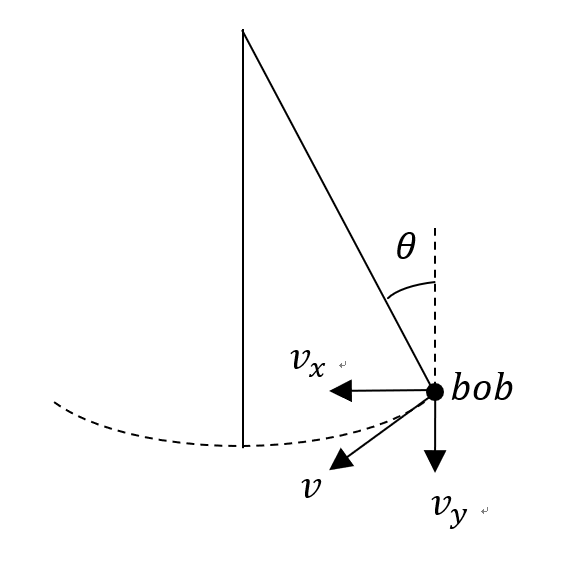
\includegraphics[scale=0.35]{2.png}
    \caption{velocity of the bob}
    \label{velocity}
\end{figure}
$$\frac{dx}{dt} = \frac{ds}{dt}cos\theta = \frac{gcos^2\theta}{k}\frac{d\theta}{dt}$$
$$\frac{dy}{dt} = \frac{ds}{dt}sin\theta = \frac{gcos\theta{sin}\theta}{k}\frac{d\theta}{dt}$$
First, we need to find the initial condition for $\theta$, $x$ and $y$ as 
$$\theta = 0 \quad x = 0 \quad y = -\frac{g}{2k}$$
We can times $dt$ on both sides of the equation and integral both sides of the equation, and we can get
\begin{equation}
    \int_0^xdx = \int_0^{\theta}\frac{gcos^2\theta}{k}d\theta
\end{equation}
\begin{equation}
    \int_{-\frac{g}{2k}}^ydy = \int_0^{\theta}\frac{gcos\theta{sin}\theta}{k}d\theta
\end{equation}
In order to calculate the integral in Eq.(11), we first use the formula 
$$cos^2\theta = \frac{1}{2}(1+cos2\theta)$$
Thus, we can get
$$x = \frac{g}{k}\int_0^{\theta}\frac{1}{2}(1+cos2\theta)d\theta$$
We now can substitute $2\theta$ with $u$, then the integral can be written as 
$$x = \frac{g}{4k}\int_0^{u}(1+cosu)du$$
The result of the integral of $x$ is that
\begin{equation}
    x = \frac{g}{4k}(2\theta+sin2\theta)
\end{equation}
Similiarly, we calculate the realtionship between $y$ and $\theta$ by the equation that 
$$cos\theta{sin}\theta = \frac{1}{2}sin2\theta$$
Thus, we can get
$$y + \frac{g}{2k} = \frac{g}{k}\int_0^{\theta}\frac{1}{2}sin2\theta{d}\theta$$
We now substitute $2\theta$ with $u$, then the integral can be written as 
$$y + \frac{g}{2k} = \frac{g}{4k}\int_0^{u}sinudu$$
The result of the integral of $y$ is that
\begin{equation}
    y = -\frac{g}{4k}(1+cos2\theta)
\end{equation}
Then we can deduce the cycloid curve from the two equations above as
\begin{equation}
    r(\theta) = (x(\theta),y(\theta)) = (\frac{g}{4k}(2\theta+sin2\theta),-\frac{g}{4k}(1+cos2\theta))
\end{equation}

\subsection{Construction of a Tautochronous Pendulum}
From the calculation in the previous part, we know that the equations for the cycloid of the bob are
$$x(\theta) = \frac{g}{4k}(2\theta+sin2\theta)$$
$$y(\theta) = -\frac{g}{4k}(1+cos2\theta)$$
First, we want to determine the radius of curvature $R$ of the parametric curve $r(\theta) = (x(\theta),y(\theta))$ at any arbitrary point P using the formula $R = \frac{1}{\kappa}$, we then using the formula from VV285 of curvature
\begin{equation}
    \kappa\circ\gamma(t) = \frac{||\gamma'(t)\times\gamma''(t)||}{||\gamma'(t)||^3}
\end{equation}
From the previous equations for $x(\theta)$ and $y(\theta)$, we differentiate them with the angel $\theta$ to get $x'(\theta)$ and $y'(\theta)$ 
$$x'(\theta) = \frac{g}{2k}(1+cos2\theta)$$
$$y'(\theta) = \frac{g}{2k}sin2\theta$$
Then we get $r'(\theta)$
$$r'(\theta) = (x'(\theta),y'(\theta)) = (\frac{g}{2k}(1+cos2\theta),\frac{g}{2k}sin2\theta)$$
Similiarly, we can differentiate the second time to get $x''(\theta)$ and $y''(\theta)$ 
$$x''(\theta) = -\frac{g}{k}sin2\theta$$
$$y''(\theta) = \frac{g}{k}cos2\theta$$
Then we get $r''(\theta)$
$$r''(\theta) = (x''(\theta),y''(\theta)) = (-\frac{g}{k}sin2\theta,\frac{g}{k}cos2\theta)$$
We take the previous results and we can get
$$\kappa\circ{r(\theta)} = \frac{||r'(\theta)\times{r''(\theta)}||}{||r'(\theta)||^3} = \frac{\frac{g^2}{2k^2}(1+cos2\theta)}{(\frac{g}{2k}\sqrt{2+2cos2\theta})^3} = \frac{k}{gcos\theta}$$
Then the curvature at any point P on the curve is calculated as
\begin{equation}
    R = \frac{1}{\kappa} = \frac{gcos\theta}{k}
\end{equation}
\begin{figure}[!htbp]
    \centering
    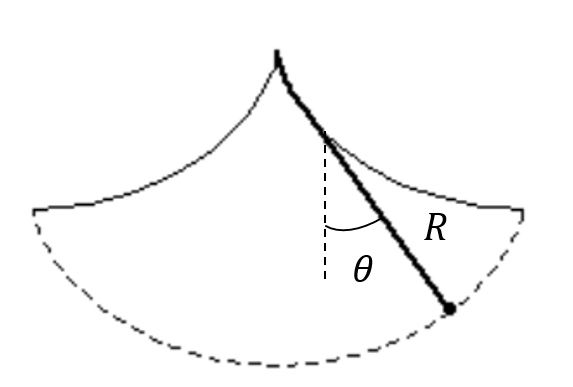
\includegraphics[scale=0.35]{3.png}
    \caption{shape of the pendulum}
\end{figure}
We now suppose the equations for the metal plates are $E(\theta) = (E_x(\theta),E_y(\theta))$. Their realtionships with $x(\theta)$ and $y(\theta)$ can be expressed as
$$E_x(\theta) = x(\theta) - Rsin\theta$$
$$E_y(\theta) = y(\theta) + Rcos\theta$$
Thus,
$$E_x(\theta) = \frac{g}{4k}(2\theta+sin2\theta) - \frac{gcos\theta{sin}\theta}{k} = \frac{g}{4k}(2\theta-sin2\theta)$$
$$E_y(\theta) = -\frac{g}{4k}(1+cos2\theta) + \frac{gcos^2\theta}{k} = \frac{g}{4k}(1+cos2\theta)$$
Then $E(\theta)$ can be expressed as
\begin{equation}
    E(\theta) = (E_x(\theta),E_y(\theta)) = (\frac{g}{4k}(2\theta-sin2\theta),\frac{g}{4k}(1+cos2\theta))
\end{equation}
It is clear that this curve is congruent to the curve of the pendulum since we can find the realtionship between $E(\theta)$ and $r(\theta)$
\begin{equation}
    E(\theta) = r(\theta - \frac{\pi}{2})+\frac{g}{4k}(\pi,2)
\end{equation}
The curve of the metal plates is simply moved from the original curve of the bob.
Apart from these, we need to make sure that the curve $E(\theta)$ satisfies the length of the line of the bob is unchanged. It means that the sum of the length of the arc and the radius of curvature will be unchanged.
We have known from the previous steps that 
$$E(0) = (0,\frac{g}{2k})$$
$$E(\frac{\pi}{2}) = (\frac{\pi{g}}{4k},0)$$
We now need to calculate the arc length from the origin point to a particular point on the curve $E(\theta)$
Since we know
$$E(\theta) = (E_x(\theta),E_y(\theta))$$
The arc length can be calculated as
\begin{equation}
    \int_0^{\theta}\sqrt{(\frac{dE_x}{d\theta})^2+(\frac{dE_y}{d\theta})^2}d\theta
\end{equation}
We first need to calculate $\frac{dE_x}{d\theta}$ and $\frac{dE_y}{d\theta}$
$$\frac{dE_x}{d\theta} = \frac{g}{2k}(1-cos2\theta)$$
$$\frac{dE_y}{d\theta} = -\frac{g}{2k}sin2\theta$$
Then the arc length is 
$$\frac{g}{2k}\int_0^{\theta}\sqrt{2-2cos\theta}d\theta$$
At this time $\theta$ is always smaller than $\frac{\pi}{2}$, meaning that $sin \theta$ is always larger than zero
Then the arc length is 
$$\frac{g}{k}\int_0^{\theta}sin\theta{d}\theta = \frac{g}{k}(1-cos\theta)$$
Then we can add the arc length and the radius of curvature to get 
\begin{equation}
    \frac{g}{k}(1-cos\theta)+\frac{gcos\theta}{k} = \frac{g}{k}
\end{equation}
which is a constant number meaning that it ensures the line of the bob unchanged, the similar result can be derived in the same way.\\
\section{Conclusion}
 Every one is familiar with pendulum since it exists everywhere in our daily life. What we normally see is the physical pendulum whose equation of rotation can be expressed as:
$$ I_s\frac{d^2\theta}{dt^2}+mgl_{cm}(sin\theta(t))=0$$
where $l_{}$ denotes the distance from the center of mass to the pivot point S and $I_s$ is the moment of inertial about the pivot point S. Since the existence of the I, it is not very convenient to study its properties. Hence, Mathematicians introduces a new term called mathematical pendulum, which is simpler with the following expression:
$$ \frac{d^2\theta(t)}{dt^2}+\frac{g}{l}sin(\theta(t))$$
We can deduce that its period is when $\theta$ is small:
$$ T\approx2\pi \frac{l_{cm}}{g}$$
Though it seems a good expression of the period since it does not depend on $\theta$, but this only works well when $\theta$ is very small. In 1659, Christiaan Huygens solved the tautochrone problem and proved that a tautochrone curve was a cyloid. This gives us a direction of construction a tautochrones pendulum.\\
~\\
Firstly, we show that tautochrone is uniqueness with the following expression of the Force exerted on the particle :
$$F(x)=-kx \qquad k>0 $$
Then we show that the tautochrone has the following expression:
$$r(\theta)=(x(\theta),y(\theta))=(\frac{g}{4k}(2\theta+sin2\theta),-\frac{g}{4k}(1+cos2\theta))$$
Clearly, our simple (mathematical) pendulum does not exactly satisfies these expressions since we use some approximation during the process. While after calculation, we find it is possible to make the motion of the pendulum into tautochrone if we add some constrain to make it move in a cycloid.
\newpage
\section{Reference}
\begin{flushleft}
$[1]$https://commons.wikimedia.org/wiki/File:Simple\_ gravity\_ pendulum.svg\\
$[2]$https://en.wikipedia.org/wiki/Pendulum\\
$[3]$https://commons.wikimedia.org/wiki/File:CyloidPendulum.png\\
$[4]$https://en.wikipedia.org/wiki/Tautochrone\_ curve\\
$[5]$R. Knoebel, A. Laubenbacher, R. Lodder, and D. Pengelley. Mathematical Masterpieces: Further Chronicles by the Explorers. Undergraduate Texts in Mathematics. Springer, 2007.\\
$[6]$ Chapter 2 Mathematical and Physical Pendulum, https://link.springer.com/chapter/10.1007 $\%$ 2F978-1-4614-3740-6\_ 2\\
$[7]$ Difference Between Simple Pendulum and Compound Pendulum, 
https://www.differencebetween.com/difference-between-simple-pendulum-and-vs-compound-pendulum/\\
$[8]$ Chapter 24 Physical Pendulum, http://web.mit.edu/8.01t/www/materials/modules/chapter24.pdf \\
$[9]$en.wikipedia.org/wiki/Arithmetic-geometric\_mean\\
$[10]$sofia.nmsu.edu/history\\
$[11]$vv285\_ project\_ 2018. https://www.umjicanvas.com/courses/576/files.
\end{flushleft}
\end{document}